%% introduction.tex
%%

%% ==============================
\chapter{Einleitung}
\label{ch:Introduction}
%% ==============================
">Ein Mensch lernt sein Leben lang."< \par

Dieser weise Spruch ist allgemein gültig. Jeder Mensch, sei es im Beruf oder im privaten Umfeld muss neue Inhalte lernen. Wie schnell er dies tut, das hängt von seinem individuellem Lerntempo ab. Damit er eine Lernhilfe erhält und neue Inhalte interessant aufbereitet, gibt es computerbasierte Hilfesysteme. Diese Hilfesysteme sind dafür da, um neue Inhalte schnell zu lernen. Wie ein solches Hilfesystem aussehen kann wird in dieser Arbeit vorgestellt. Die neuen Lerninhalte beziehen sich auf eine spezielle Software, welche bei der Ausschreibung des Seminarthemas vorgeschrieben wurde. Diese Software soll im Folgenden kurz erläutert werden.




\section{CAS Campus}
Die Zielsoftware, worauf unsere spätere Empfehlung basiert, ist die Software CAS Campus. Diese Software ist von der CAS Software AG aus Karlsruhe. Das Ziel der Software ist es einen kompletten Student-Lifecycle (siehe Abbildung \ref{img1:stdLife}) nachzubilden. Der Lifecycle beginnt mit der Bewerbung des Studenten an einer Hochschule und endet mit dem Alumni Zustand. Bevor er zu dem Alumni-Zustand kommt, muss er einige Stationen begleiten. Auf dem Weg zum Abschluss werden einige Prozesse durchlaufen und der Student hat sehr viel Verwaltungsaufwand zu erledigen. Weiterhin wird er mit vielen Personen während seines Studiums in Berührung kommen. Diese Prozesse und Vorgänge versucht die Software bestmöglich abzubilden, indem Sie mehrere Plattformen zur Verwaltung und Steuerung anbietet. Die Software wird von mehreren Personen an einer Hochschule verwendet. Diese Personas werden in Kapitel \ref{ch:Content1} weiter erläutert und vorgestellt. \footnote{Quelle: http://www.cas-education.de/fuer-hochschulen/cas-campus.html aufgerufen am 18.07.2015}
\begin{figure}[ht]
\begin{center}
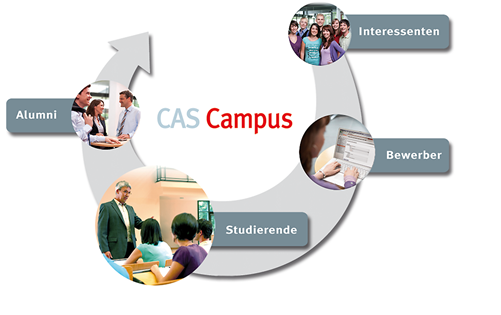
\includegraphics[width = 0.5\textwidth]{casCampus.png}
\caption{Student-Lifecycle}
\label{img1:stdLife}
\end{center}
\end{figure} 

\section{Weiteres Vorgehen}
Im folgenden Text wird zuerst der aktuelle Status-Quo in Sachen Lernen und Online-Hilfe erläutert. Darauf aufbauend wird erklärt, was genau Adaptiv für unsere Arbeit bedeutet und worauf wir unseren Schwerpunkt beziehen. Zur besseren Einführung in die Thematik werden die Nutzer und deren Probleme in Form von Personas vorgestellt. Diese Nutzer werden anschließend Klassifiziert, damit bessere Lösungsansätze gefunden werden können. Anhand der Klassifizierung werden wir unsere Lösungsansätze vorstellen, diese kritisch bewerten und eine anschließende Empfehlung daraus generieren. Zum Abschluss der Arbeit möchten wir ein kleines Fazit mit Ausblick auf ein weiteres Vorgehen bei der Arbeit geben.


